\documentclass[conference]{IEEEtran}
\usepackage{amsmath,amssymb}
\usepackage{graphicx}
\usepackage{booktabs}
\usepackage{cite}
\usepackage{tikz}
\usetikzlibrary{arrows.meta,positioning,fit}
\usepackage{xurl}
\usepackage[hidelinks]{hyperref}
% Generated by paper/figures.py. Do not edit.
\newcommand{\RunsMain}{1350}
\newcommand{\SeedsMain}{10}
\newcommand{\CalibratedGain}{0.15}
\newcommand{\CustAufls}{11.1}
\newcommand{\StagesAufls}{0.56}
\newcommand{\EnsAufls}{1.73}
\newcommand{\UnservedAufls}{0.82}
\newcommand{\NadirAufls}{49.475}
\newcommand{\CustHeur}{12.8}
\newcommand{\StagesHeur}{0.00}
\newcommand{\EnsHeur}{0.00}
\newcommand{\UnservedHeur}{0.54}
\newcommand{\NadirHeur}{49.595}
\newcommand{\CustEdge}{11.6}
\newcommand{\StagesEdge}{0.00}
\newcommand{\EnsEdge}{0.00}
\newcommand{\UnservedEdge}{1.13}
\newcommand{\NadirEdge}{49.760}
\newcommand{\CustNpmrd}{1.1}
\newcommand{\StagesNpmrd}{0.00}
\newcommand{\EnsNpmrd}{0.00}
\newcommand{\UnservedNpmrd}{0.19}
\newcommand{\NadirNpmrd}{49.542}
\newcommand{\CustHybrid}{1.4}
\newcommand{\StagesHybrid}{0.00}
\newcommand{\EnsHybrid}{0.00}
\newcommand{\UnservedHybrid}{0.22}
\newcommand{\NadirHybrid}{49.546}
\newcommand{\CustNpVsAufls}{-10.0}
\newcommand{\CustNpVsAuflsLo}{-11.1}
\newcommand{\CustNpVsAuflsHi}{-8.8}
\newcommand{\CustNpVsAuflsP}{4.1e-28}
\newcommand{\CustNpVsHeur}{-11.6}
\newcommand{\CustNpVsHeurLo}{-12.9}
\newcommand{\CustNpVsHeurHi}{-10.4}
\newcommand{\CustNpVsHeurP}{2.6e-31}
\newcommand{\CustHyVsAufls}{-9.7}
\newcommand{\CustHyVsAuflsLo}{-10.8}
\newcommand{\CustHyVsAuflsHi}{-8.6}
\newcommand{\CustHyVsAuflsP}{4.3e-28}
\newcommand{\CustHyVsHeur}{-11.4}
\newcommand{\CustHyVsHeurLo}{-12.6}
\newcommand{\CustHyVsHeurHi}{-10.1}
\newcommand{\CustHyVsHeurP}{2.5e-31}
\newcommand{\CustHyVsEdge}{-10.3}
\newcommand{\CustHyVsEdgeLo}{-10.9}
\newcommand{\CustHyVsEdgeHi}{-9.6}
\newcommand{\CustHyVsEdgeP}{4.2e-46}
\newcommand{\WorstStagesHy}{0.00}
\newcommand{\WorstCustHy}{3.4}
\newcommand{\WorstStagesNp}{1.00}
\newcommand{\WorstCustNp}{24.1}
\newcommand{\WorstLatency}{2.0}
\newcommand{\WorstLoss}{40}
\newcommand{\CalTestErrMax}{0.007}
\newcommand{\CalDefaultErrMin}{0.32}
\newcommand{\CalDefaultErrMax}{0.43}
\newcommand{\CalGainMax}{0.17}


\begin{document}

\title{Nadir-Predictive, Consent-Constrained Appliance Relief\\Beneath Under-Frequency Load Shedding:\\A Calibrated Study for the Indian Grid}

\author{\IEEEauthorblockN{Author One, Author Two, Author Three}
\IEEEauthorblockA{Department of Computer Science and Engineering, RV College of Engineering, Bengaluru, India\\
\{author\}@rvce.edu.in}}

\maketitle

\begin{abstract}
When a large generator trips, automatic under-frequency load shedding (AUFLS) disconnects whole distribution feeders, interrupting every customer on them, including clinics and water services that share those feeders. We study whether consenting households' flexible appliances can supply just enough relief, early enough, to keep frequency above the first AUFLS stage. We propose Nadir-Predictive Minimum-Relief Dispatch (NP-MRD): the controller estimates the power deficit from the swing equation, predicts the frequency trajectory with the Anderson--Mirheydar system frequency response model including governor limits, finds the smallest relief that keeps the predicted nadir above the protection threshold, and selects appliances with a covering knapsack that first minimises customers interrupted, then guaranteed deferred energy, then thermal discomfort. To tolerate communication delay and loss, a hybrid variant pre-arms nested appliance sets for a ladder of contingency sizes, triggered locally by measured rate of change of frequency, as in special protection schemes. The governor gain is calibrated, leave-one-event-out, to two published Indian events (test-event nadir error at most \CalTestErrMax~Hz, against \CalDefaultErrMin--\CalDefaultErrMax~Hz for textbook parameters). Across \RunsMain{} paired simulations, NP-MRD interrupts \CustNpmrd{} customers per event on average against \CustAufls{} for AUFLS alone and \CustHeur{} for a frequency-threshold heuristic, with no AUFLS operation in the reported cases. With \WorstLatency~s command latency and \WorstLoss\% packet loss, the hybrid operates \WorstStagesHy{} AUFLS stages on average against \WorstStagesNp{} for central dispatch. The study is simulation-based; limitations are stated explicitly.
\end{abstract}

\begin{IEEEkeywords}
under-frequency load shedding, demand response, frequency nadir, system frequency response model, special protection scheme, digital twin
\end{IEEEkeywords}

\section{Introduction}
Indian regional grids rely on AUFLS relays that open pre-assigned feeders at 49.4, 49.2, 49.0 and 48.8~Hz~\cite{srpc2024}. Two recent events, a 7{,}120~MW loss in Rajasthan on 15 May 2023~\cite{nerpc2023} and an 8{,}963~MW loss near Khavda on 13 May 2026~\cite{erpc2026}, both drew frequency to about 49.4~Hz and operated AUFLS. Feeder-level shedding is coarse: every customer on a feeder is interrupted regardless of what they are using, and essential services on mixed feeders are interrupted with them.

Household appliances can respond to frequency~\cite{short2007,molina2011}, and load-side control can contribute to primary response~\cite{zhao2014}. Using intelligent appliances so that UFLS operates less, or not at all, has also been proposed~\cite{wang2016}. Utility demand response in India, such as the Tata Power--AutoGrid programmes, addresses peak reduction over minutes to hours~\cite{tatapower}. This paper asks a narrower question: in the seconds after a contingency, what is the \emph{smallest} set of consenting appliances whose curtailment prevents AUFLS from operating, which customers should supply it, and how robust is that answer to imperfect communication?

Contributions:
\begin{enumerate}
\item NP-MRD, a controller that computes minimum appliance relief from a predicted frequency nadir using the Anderson--Mirheydar SFR model~\cite{anderson1990} with governor dead band and reserve limits, and selects appliances by a lexicographic covering knapsack over customers interrupted, guaranteed deferred energy and thermal slack.
\item A hybrid scheme that pre-arms nested minimum-relief sets for a ladder of contingency sizes and triggers them locally on measured RoCoF, following the structure of special protection schemes~\cite{anderson1996}, with central refinement over an impaired channel.
\item A leave-one-event-out calibration of the primary-response gain to two Indian events, and paired experiments on inertia, contingency size, enrollment, latency and packet loss, released with the open simulator and a campus digital twin.
\end{enumerate}

\section{Related work}
\emph{Appliances instead of feeder shedding.} Wang et al.~\cite{wang2016} coordinate intelligent home appliances with conventional UFLS in a cyber-physical setting so that appliance response replaces part of the passive shedding; field trials of frequency-responsive water heaters and dryers found responses largely unnoticed by owners~\cite{pnnl2014}. Decentralised threshold relays~\cite{short2007,molina2011} and smart-meter or appliance UFLS in microgrids~\cite{xu2023} act on fixed frequency settings rather than a computed relief requirement.
\emph{Sizing the relief.} Terzija~\cite{terzija2006} estimated the disturbance from the swing equation to adapt UFLS; analytic SFR models have been used offline to size the minimum shed~\cite{elzawawy2019}, and Elsaadany et al.~\cite{elsaadany2025} periodically re-optimise UFLS relay set-points with a reduced-order model including governor limits, noting that SFR-based settings can under-estimate the required shedding at low inertia. Panagi et al.~\cite{panagi2026} procure fast frequency response from EV and heat-pump fleets day-ahead to keep the nadir above UFLS thresholds.
\emph{Gap.} These works size feeder-level shedding or procure aggregate capacity. We did not find an approach that (i) computes, online, the minimum \emph{appliance-level} relief from a limiter-aware nadir prediction and assigns it customer-first under compressor lockout and comfort constraints, or (ii) pre-arms nested appliance sets for a ladder of contingency sizes with model-derived RoCoF triggers and quantifies the robustness to command latency and loss, or (iii) calibrates such a study to Indian events. These three elements are the contribution; the use of appliances to avoid UFLS is not.

\section{System model}
\subsection{Frequency dynamics}
We use the reheat SFR model of~\cite{anderson1990}: $2H\,\dot{\omega}=\Delta P_m-\Delta P_d-D\,\Delta\omega$ with $\Delta P_m=\frac{K_m}{R}\frac{1+F_HT_Rs}{1+T_Rs}(-\Delta\omega)$, a governor dead band of 30~mHz and reserve limits of $+0.15$/$-0.30$~pu, integrated by RK4 at 50~ms. The closed-form nadir of~\cite{anderson1990} matches the integrated plant to within $10^{-3}$~Hz when the limiters are inactive (unit test in the released code). $T_R=8$~s, $F_H=0.3$, $R=0.05$, $D=1$ follow~\cite{anderson1990}; $K_m$ is calibrated (Section~\ref{sec:cal}).

\subsection{Protection, fleet and appliances}
The AUFLS reference uses the SRPC stages and 5/6/7/7\% relief~\cite{srpc2024}, applied to whole modelled feeder blocks with a 100~ms dwell; protected facilities are on exempt feeders. The area has 500 buildings (houses, apartments, shops, clinics, a cold-chain store and a water pumping station). Appliance ratings follow utility calculator values; flexible appliances are room AC (with 180~s compressor restart lockout), storage water heaters and EV chargers. Only appliances in enrolled buildings, with consent, are eligible; critical and essential loads never are. Thermal states use the first-order equivalent-thermal-parameter model with parameters from~\cite{mathieu2013}; comfort is reported as degree-minutes outside the band.

\section{Nadir-predictive minimum-relief dispatch}
\subsection{Deficit estimate and prediction}
Every 0.5~s the controller solves the swing equation for the net deficit, $\hat{P}=P_m-D\Delta\omega-2H\dot{f}/f_0$~\cite{kundur1994,inoue1997,terzija2006}, using an observer copy of the governor state driven by the 20~sample/s frequency stream (a PMU reporting rate~\cite{c37118}). It then integrates the same SFR model, limiters included, from the present state for a vector of candidate reliefs and returns the smallest relief $R^\ast$ whose predicted minimum frequency stays at or above $49.40+m$~Hz, with margin $m=0.05$~Hz. Relief is capped at the estimated deficit, since more cannot raise the nadir without creating a surplus.

\subsection{Appliance selection}
Given $R^\ast$, binary $x_i$ selects appliance $i$ (power $p_i$) and $z_b$ marks a newly interrupted customer $b$:
\begin{align}
\min\; & \textstyle\sum_b z_b + \epsilon_1\sum_i \tilde{e}_i x_i + \epsilon_2 \sum_i \rho_i x_i\\
\text{s.t.}\; & \textstyle\sum_i p_i x_i \ge R^\ast,\quad x_i \le z_{b(i)},\quad x_i,z_b\in\{0,1\},
\end{align}
where $\tilde{e}_i$ is the normalised guaranteed deferred energy $p_iL_i$ ($L_i$ the minimum off time) and $\rho_i$ the position in the comfort band (priority stack~\cite{lu2012}; least laxity for EVs~\cite{xu2016}). Weights $\epsilon_1=1/(n+1)$ and $\epsilon_2=\epsilon_1/(n+1)$ make the objective lexicographic. The first term counts customers as in SAIFI~\cite{ieee1366}. The problem is solved with HiGHS; small instances are verified against exhaustive search.

\subsection{Restoration}
Curtailed appliances are restored in order of comfort urgency when the predicted minimum frequency including the restart pickup (rated power times inrush ratio, held conservatively) remains above $49.40+m+0.05$~Hz.

\subsection{Hybrid: pre-armed relief with local triggering}
Before any event the controller computes, with the same predictor from equilibrium, the minimum relief for contingency sizes $P_k=0.01k$~pu, $k=1\ldots30$, assuming relief begins after a 0.25~s local detection delay, and selects nested sets with the same knapsack. The set added at level $k$ is needed for every contingency larger than $P_{k-1}$, so each appliance is armed with the RoCoF the model predicts over the first 0.2~s for $P_{k-1}$. Arming is broadcast every second and re-planned every minute over the same impaired channel. Appliances trip locally when their own RoCoF measurement is below the armed value; NP-MRD then refines and restores centrally.

\begin{figure}[t]
\centering
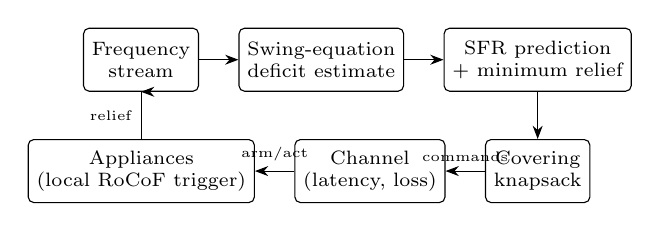
\begin{tikzpicture}[font=\scriptsize, box/.style={draw, rounded corners=2pt, align=center, minimum height=0.8cm, inner sep=3pt}, >=Stealth]
\node[box] (pmu) {Frequency\\stream};
\node[box, right=0.5cm of pmu] (obs) {Swing-equation\\deficit estimate};
\node[box, right=0.5cm of obs] (pred) {SFR prediction\\+ minimum relief};
\node[box, below=0.6cm of pred] (ks) {Covering\\knapsack};
\node[box, left=0.5cm of ks] (ch) {Channel\\(latency, loss)};
\node[box, left=0.5cm of ch] (dev) {Appliances\\(local RoCoF trigger)};
\draw[->] (pmu) -- (obs); \draw[->] (obs) -- (pred); \draw[->] (pred) -- (ks);
\draw[->] (ks) -- node[above]{\tiny commands} (ch); \draw[->] (ch) -- node[above]{\tiny arm/act} (dev);
\draw[->] (dev.north) |- node[pos=0.25,left]{\tiny relief} (pmu.south);
\end{tikzpicture}
\caption{NP-MRD and the hybrid scheme. Pre-armed appliances act locally; the central loop refines.}
\label{fig:arch}
\end{figure}

\section{Calibration to Indian events}\label{sec:cal}
Public event reports give the loss, the pre-event frequency and the nadir but not the system base or inertia. We therefore sweep the base (200 and 250~GW) and $H$ (4 and 5~s), fit $K_m$ on one event by root-finding on the simulated nadir (AUFLS active, initial frequency as reported), and test on the other event. Test-event nadir errors are at most \CalTestErrMax~Hz; textbook $K_m=0.95$ errs by \CalDefaultErrMin--\CalDefaultErrMax~Hz. Fitted gains are at most \CalGainMax. Because both observed nadirs were arrested by AUFLS near 49.4~Hz, the data bound the effective gain from above rather than identify it; we use $K_m=\CalibratedGain$ and report textbook parameters as a sensitivity.

\section{Experiments}
Each run simulates 270~s with a step loss of generation at 5~s and recovery from 45~s over 30~s. Main comparison: five policies (AUFLS only, the original frequency-threshold heuristic, decentralised edge relays~\cite{molina2011}, NP-MRD, hybrid) $\times$ $H\in\{5,3,2\}$~s $\times$ loss $\in\{2,3.5,5\}$\% $\times$ enrollment $\in\{25,50,100\}$\% $\times$ \SeedsMain{} seeds, paired on seed. Seeds vary enrollment, ownership and use; intervals describe modelled variation only.

\begin{figure}[t]
\centering
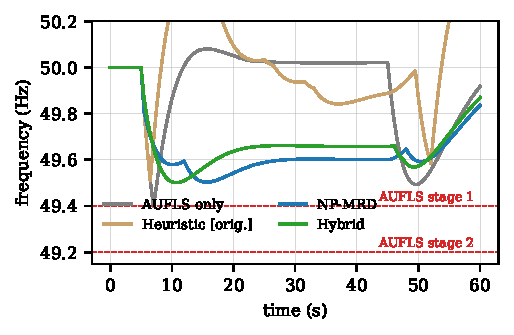
\includegraphics[width=\columnwidth]{figures/trajectories.pdf}
\caption{Frequency at $H=3$~s, 5\% loss, calibrated governor gain.}
\label{fig:traj}
\end{figure}

\begin{figure*}[t]
\centering
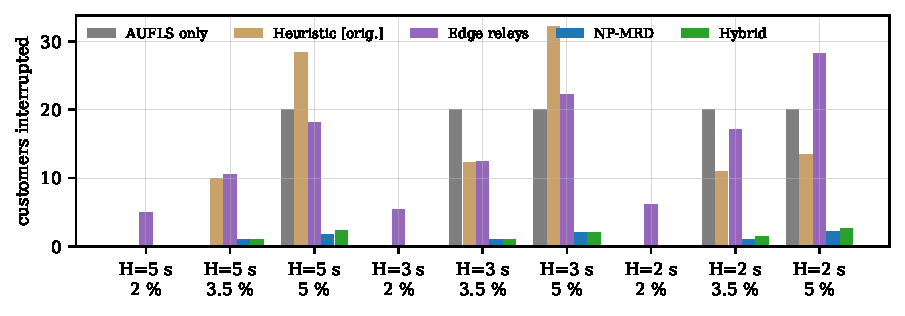
\includegraphics[width=\textwidth]{figures/customers.pdf}
\caption{Customers interrupted per event (mean over seeds, full enrollment). AUFLS-only interruptions are whole feeder blocks.}
\label{fig:customers}
\end{figure*}

\subsection{Main comparison}
Table~\ref{tab:main} and Fig.~\ref{fig:customers} summarise the outcomes. Paired over all main cases, NP-MRD changes customers interrupted by \CustNpVsAufls{} [\CustNpVsAuflsLo, \CustNpVsAuflsHi] relative to AUFLS only (Wilcoxon $p=\CustNpVsAuflsP$) and by \CustNpVsHeur{} [\CustNpVsHeurLo, \CustNpVsHeurHi] relative to the heuristic ($p=\CustNpVsHeurP$). The heuristic over-relieves: it sheds on a fixed threshold in proportion to the frequency error, which raises the nadir beyond what protection requires and drives frequency above 50~Hz (Fig.~\ref{fig:traj}).

\begin{table}[t]
\centering
\caption{Means over all main-comparison runs. Cust.: customers interrupted; Stages: AUFLS stages operated; ENS: critical energy not served.}
\label{tab:main}
\footnotesize
\setlength{\tabcolsep}{4pt}
\begin{tabular}{lrrrr}
\toprule
Policy & Cust. & Stages & ENS (Wh) & Nadir (Hz)\\
\midrule
AUFLS only & \CustAufls & \StagesAufls & \EnsAufls & \NadirAufls\\
Heuristic & \CustHeur & \StagesHeur & \EnsHeur & \NadirHeur\\
Edge relays & \CustEdge & \StagesEdge & \EnsEdge & \NadirEdge\\
NP-MRD & \CustNpmrd & \StagesNpmrd & \EnsNpmrd & \NadirNpmrd\\
Hybrid & \CustHybrid & \StagesHybrid & \EnsHybrid & \NadirHybrid\\
\bottomrule
\end{tabular}
\end{table}

\subsection{Communication impairments}
Fig.~\ref{fig:comm} varies command latency (0--2~s, jitter of half the latency) and packet loss (0--40\%) at $H=3$~s and 5\% loss. Central NP-MRD loses its benefit once latency approaches the time to the nadir, because relief arrives after frequency has crossed the first stage. At 2~s latency it operates one AUFLS stage and interrupts \WorstCustNp{} customers on average. The hybrid's pre-armed sets act within the local detection delay regardless of the channel, so the central loop only refines: it operated no AUFLS stage in any tested latency--loss combination and interrupted at most \WorstCustHy{} customers in the worst case. With zero latency but 40\% loss, lost central commands caused NP-MRD to re-select appliances and, in some seeds, to arrive late; pre-arming removes this sensitivity.

\begin{figure*}[t]
\centering
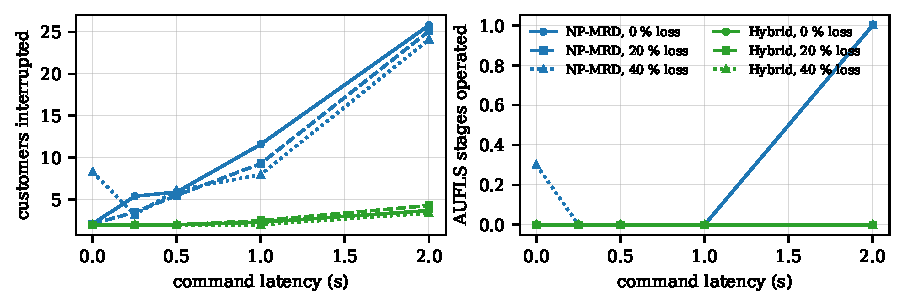
\includegraphics[width=\textwidth]{figures/communication.pdf}
\caption{Effect of command latency and packet loss ($H=3$~s, 5\% loss).}
\label{fig:comm}
\end{figure*}

\subsection{Margin and inertia-estimate error}
Fig.~\ref{fig:margin} shows the trade-off between the protection margin $m$ and customers interrupted: a larger margin raises the nadir at the cost of more interrupted customers. With the operator's inertia estimate 15--30\% too high, NP-MRD still avoided AUFLS; with it 30\% too low, the controller under-predicted the decline and AUFLS operated in two of ten seeds, so inertia estimation (e.g.~\cite{inoue1997}) is a prerequisite for deployment.

\subsection{Sensitivity: textbook governor response}
With $K_m=0.95$ and larger contingencies (10\% and 18\%), NP-MRD and the hybrid again avoided AUFLS with several times fewer customers than the heuristic. At 18\% loss, however, they deferred more total energy than the heuristic, because the knapsack prefers few large appliances (EV chargers) that remain curtailed until generation recovers. Customer count and deferred energy are therefore competing objectives; the lexicographic order is a design choice that a utility could reverse.

\begin{figure}[t]
\centering
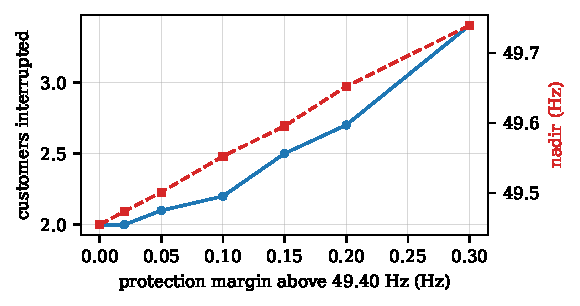
\includegraphics[width=\columnwidth]{figures/margin.pdf}
\caption{Protection margin trade-off for NP-MRD ($H=3$~s, 5\% loss).}
\label{fig:margin}
\end{figure}

\section{Campus digital twin}
The simulator drives a browser-based twin of the RVCE campus. Building footprints come from Microsoft's machine-detected footprints (ODbL); annual energy is estimated from floor area and the Bureau of Energy Efficiency benchmark for institutes in the moderate climate zone (129~kWh/m$^2$/yr)~\cite{bee_epi}. Building names, uses and floor counts are explicit defaults to be replaced by verified data. The twin shows the frequency, the predicted nadir and the audited reason for every curtailment.

\section{Limitations}
The study is single-area with no voltage or power-flow constraints, and the predictor shares the SFR structure of the simulated plant; Elsaadany et al.~\cite{elsaadany2025} show that SFR-type models can under-estimate required relief at low inertia, so a higher-fidelity plant is needed to confirm the margins reported here. Only two field events are available and both nadirs were arrested by AUFLS, so the governor gain is bounded rather than identified. Appliance response, communication and comfort are models; the campus loads are benchmark estimates. No field trial was performed. Frequency is held near 49.5~Hz by the minimum-relief policy until generation recovers, which assumes secondary control restores frequency afterwards.

\section{Conclusion}
Predicting the nadir and asking for the minimum relief that keeps frequency above the first AUFLS stage avoided feeder shedding in the reported cases while interrupting far fewer customers than either AUFLS or a threshold heuristic. Pre-arming that relief with local RoCoF triggering kept the benefit under command latency and packet loss. Field validation with measured appliance response and utility event data is the next step.

\bibliographystyle{IEEEtran}
\bibliography{references}
\end{document}
